\chapter{Discussion}\label{disc}
\thispagestyle{plain}
In this chapter a deeper analysis of the results from chapter \ref{chap3} are presented in order to try to understand the behavior of the models and compare their performances. A comparison of the results obtained with the models used in this thesis to the model presented by \cite{Farinotti2019} will also be presented as it is interesting to compare statistical based models as those deriving from machine learning algorithm to the physical based ones from  \cite{Farinotti2019}.

\section{Machine learning models performances}\label{MLcomp}

\begin{figure}[p]
	\centering		  
	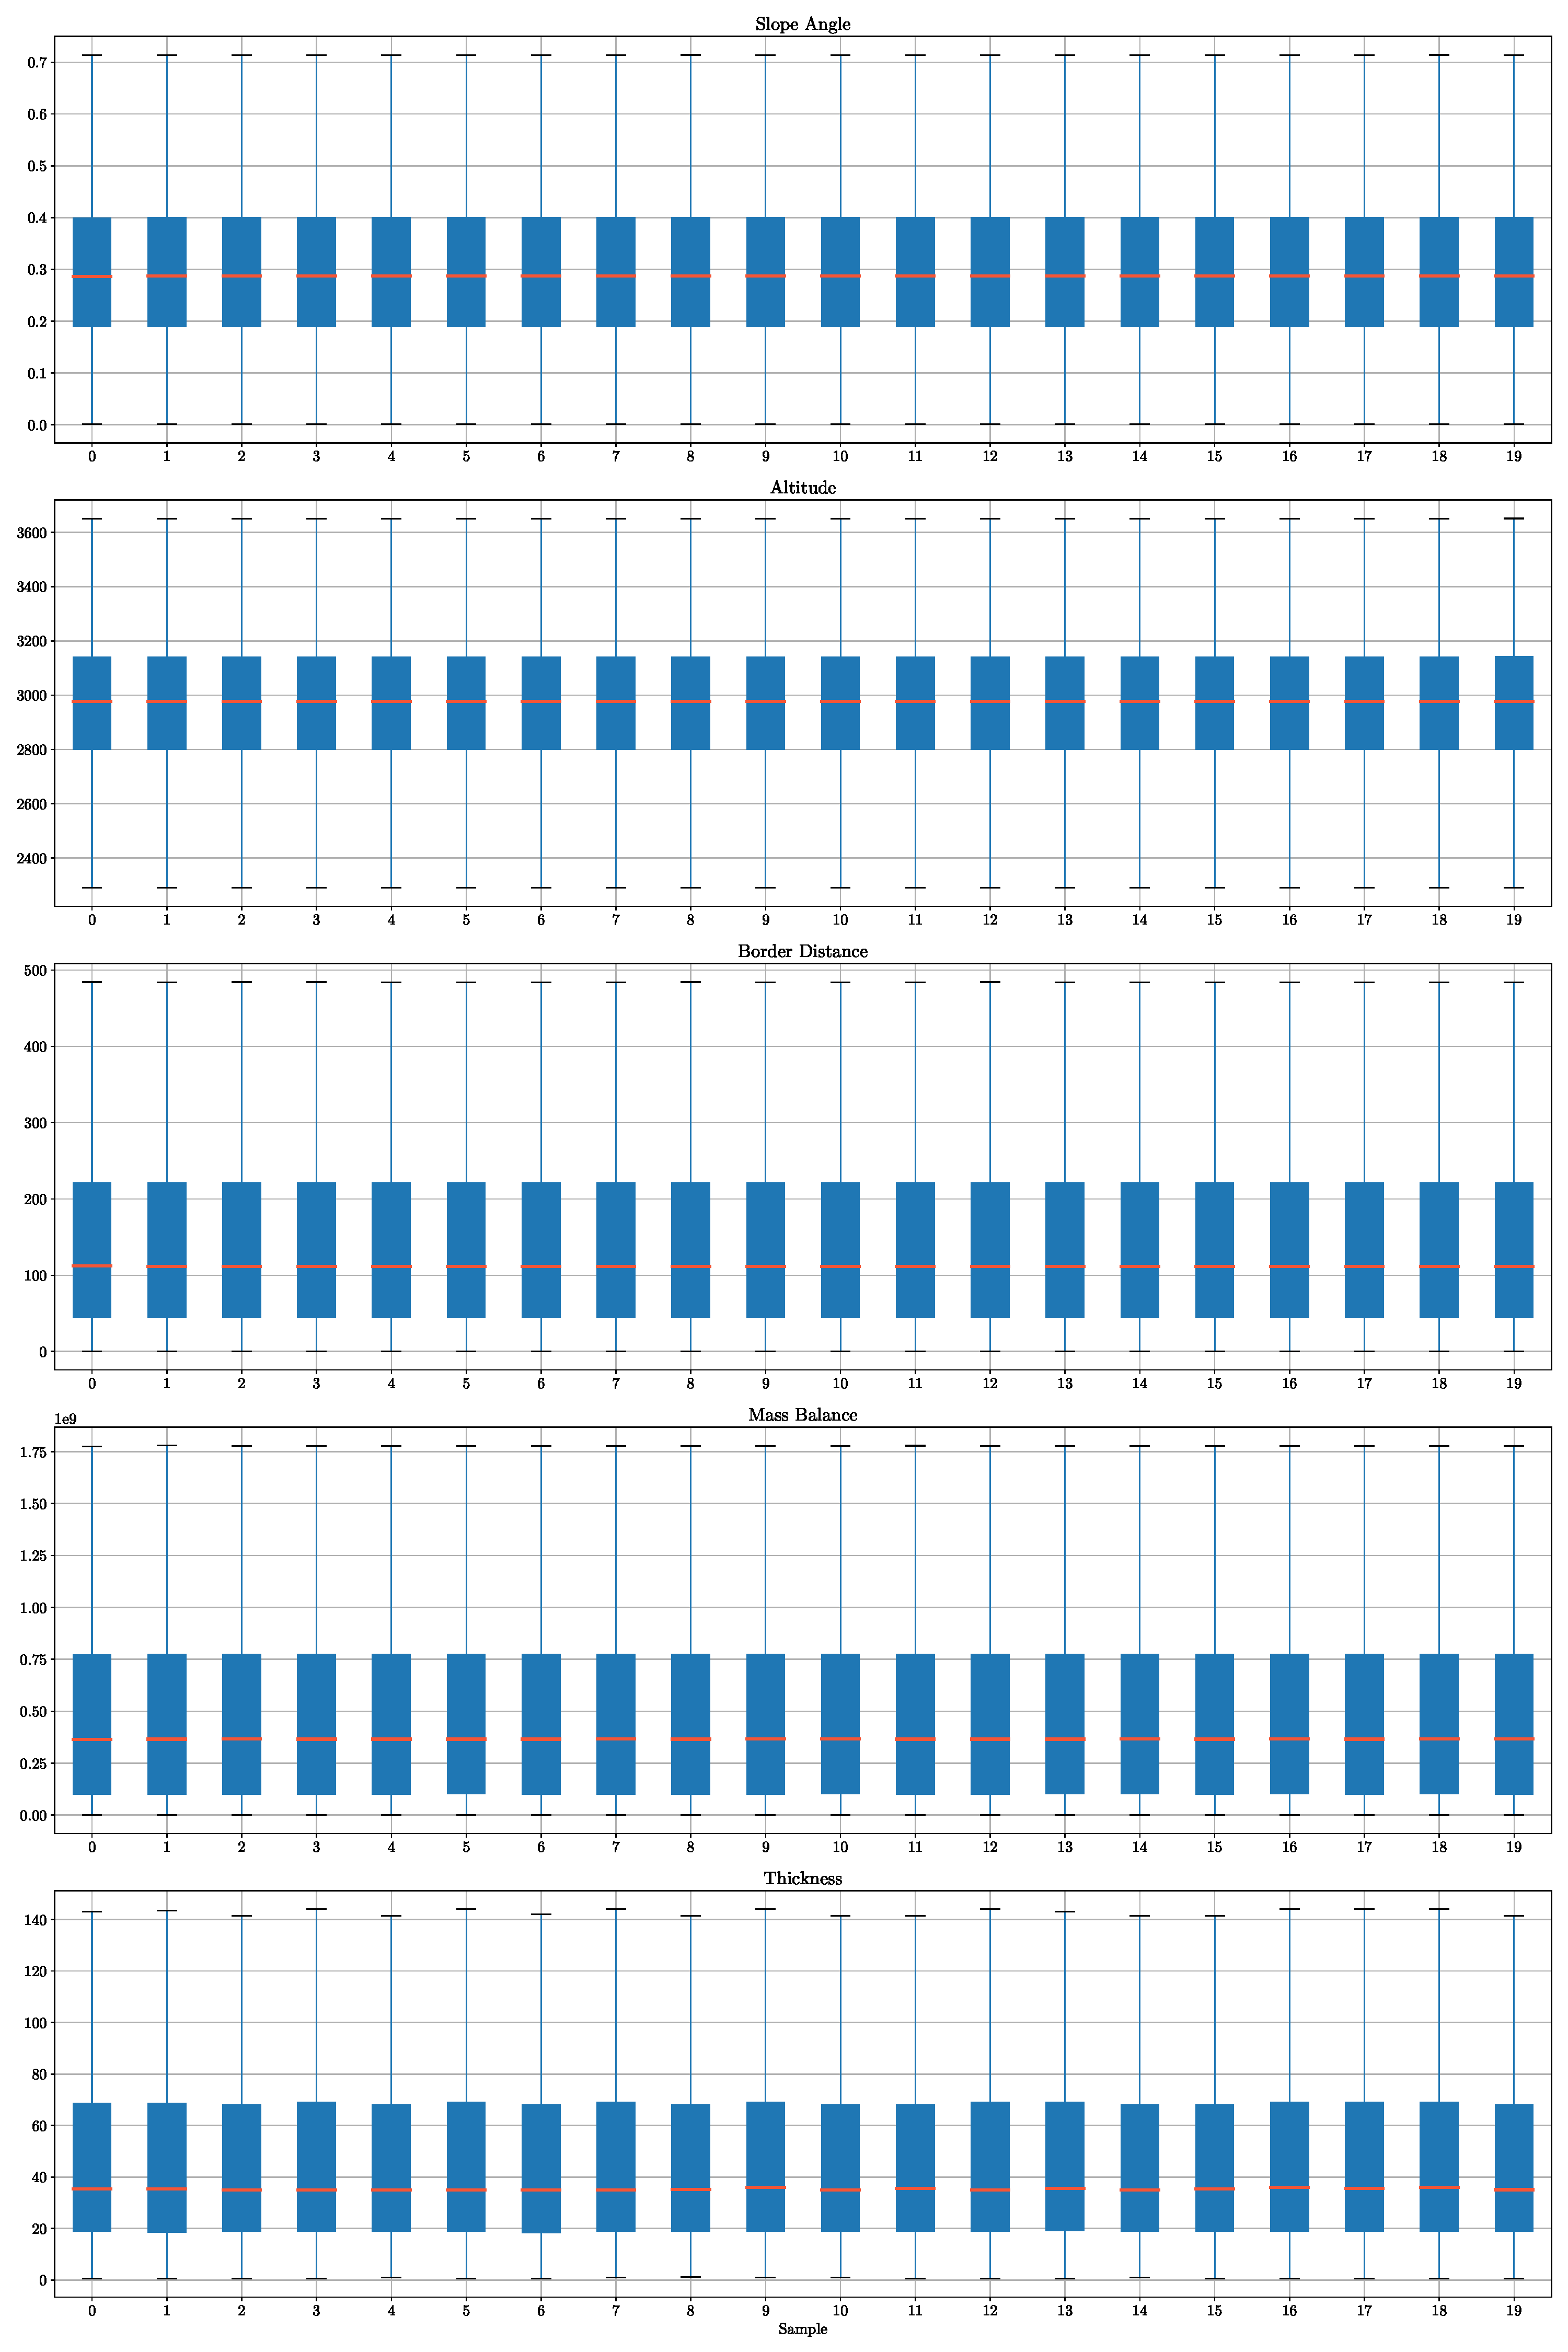
\includegraphics[width=1.\textwidth]{figures/samples_distribution.pdf}
	\caption{Distribution of the attributes used for training the models along the different sub-samples}
	\label{fig:distribution}
\end{figure}

\subsection{Score}\label{disc-score}

One of the easiest approaches to infer the reliability of a model is to check how good is the model at predicting known values. When doing this for a model coming from a machine learning algorithm one needs to be careful at not over-fitting the model, i.e. having a model which is very good at making predictions for data points coming from the data used for training the model but very bad at predicting values for data not used for training. For this reason the models have all been trained using 20 different sub-samples and checking the how good they were doing when making predictions using data left out from the sub-samples used for training.
None of the three models used seem to do a very good job at predicting the ice thickness based on their scores. In the best case in fact the support vector regression had an average score of 0.55 but with a high variance due to sub-samples 5, 14 and 19 having a much lower score. Even the best performing of the trained models which still was one of the support vector regression models trained only had a score just above 0.6. This means that the best model only explain 60\% of the variance of the thickness observations fro the GlaThiDa database.

\begin{figure}[!tp]
	\centering		  
	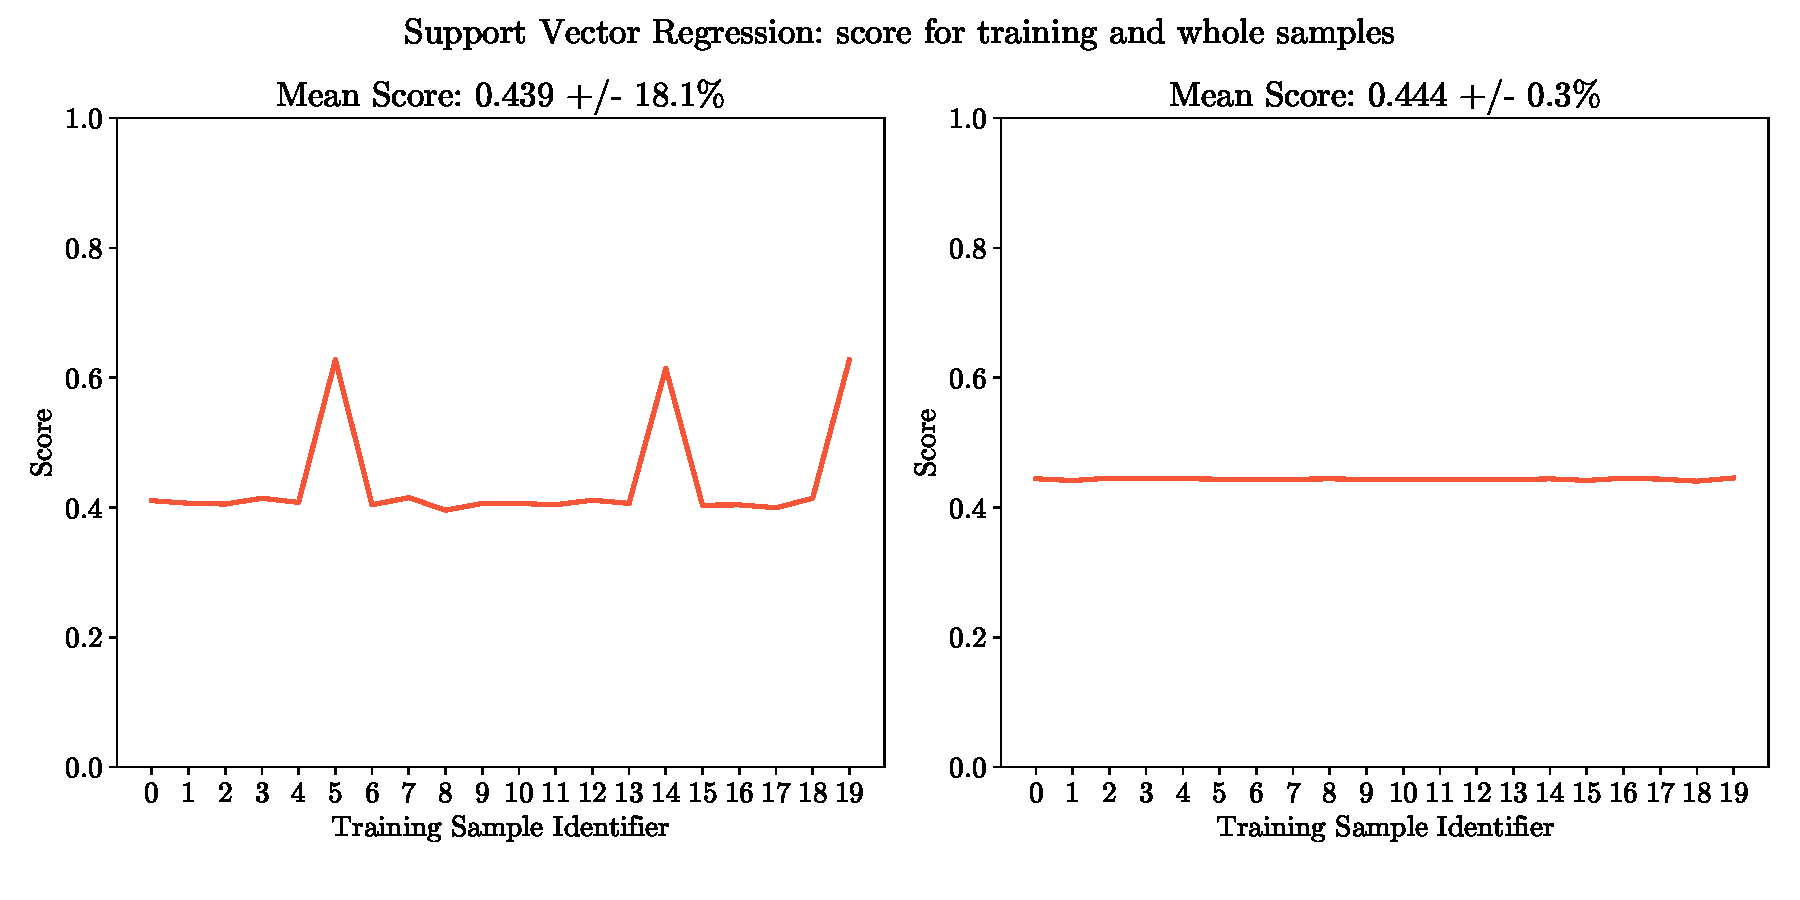
\includegraphics[width=1.\textwidth]{figures/SVR_score_tr.pdf}
	\caption{Support Vector Regression: on the left score achieved by the models trained with the different sub-samples calculated using the training sample instead if the testing sample; on the right the score computed on the whole sub-sample (train and testing data)}
	\label{fig:train-score}
\end{figure}

Interestingly all the models have drops in performance for the sub-samples  5, 14 and 19. A possible explanation of this behavior could be explained by the fact that the sub-sample used for training these models could be missing some data points in the training set which were essential for training a model leading to accurate predictions. If for example those sub-sample had a very different value distribution in any of the attributes used for training compared to the distribution of the whole data-set, it could lead to a biased model not capable of making accurate predictions. This, however difficult to compute exactly, doesn't seem to be the case when looking at Fig. \ref{fig:distribution} showing box-plots of the data distribution for each of the attributes and sample.

\begin{table}[!b]
	\centering
	\caption{Score for the three models used when training them with all the data available from the GlaThiDa.}
	\begin{tabular}{|c|c|c|c|}
		\hline 
		Linear Regression&Random Forest&Support Vector Regression \\
		\hline
		0.32&0.57&0.45 \\
		\hline
	\end{tabular}
	\label{tb:all-score}
\end{table}

Fig. \ref{fig:train-score} shows the score achieved by the support vector machine by the models trained with the different sub-samples. On the right the score was calculated only on the sample used for training in each sub-sample. This in contrast with the results shown in chapter \ref{chap3} which showed the score computed on the data not used for training in each sub-sample. The left chart shows how the highest scores are achieved for sub-samples 5, 14, and 19. Those are the same sub-samples which were showing the lowest scores when computing the score on the testing samples. On the right we can see the scores computed on the whole data-set. The scores are almost constant throughout the sub-samples. All this could be indicating that the reason for the drop in scores showed in chapter \ref{chap3} could be attributed to the fact that the samples left out for testing are particularly difficult to compute for the model. Similar results can be shown also for the linear regression model and for the random forest regression.

Even if the random forest model achieved an average score lower than the one achieved by the support vector machine one when training them with the sub-samples, the score of the random forest regression achieved when training it on the whole sample is the highest among the models used (see Tab. \ref{tb:all-score}). This score is calculated on the same data used for training the model. It could then be prone to overfitting, in particular for the random forest regression which already showed some sign of it when looking at the scores for the different sub-samples.

\subsection{Volume Distribution}\label{disc-vol-dist}
The score is a great value to assess how well the model replicates known data. However for glaciers looking at the distribution of the ice thickness over the glacier surface in a map is also important. Clearly both the random forest and the support vector regression models have problems in computing large values of ice thicknesses as showed in Fig. \ref{fig:rfr-map} and Fig. \ref{fig:svr-map}. For the random forest regression it seems like there is a an upper ice thickness threshold after which the model computes a constant ice thickness value. This is why the ice thickness distribution maps show large zones of constant ice thickness towards the middle of the glaciers. This can also be confirmed when looking at Fig. \ref{fig:rfr-pdp} which shows that after a certain threshold the model predicts no ice thickness change for any change in any feature value. This is clearly a downside of this model which can only predict values within the range of the values found in the training data-set. To improve the prediction for the model for large ice thickness values one could increase the maximum depth of the trees and the minimum number of samples needed for splitting at the node. This would make the model able to better distinguish values for outliers. However there will always be an upper and lower limit for values predicted by the model.

\begin{figure}[!tp]
	\centering		  
	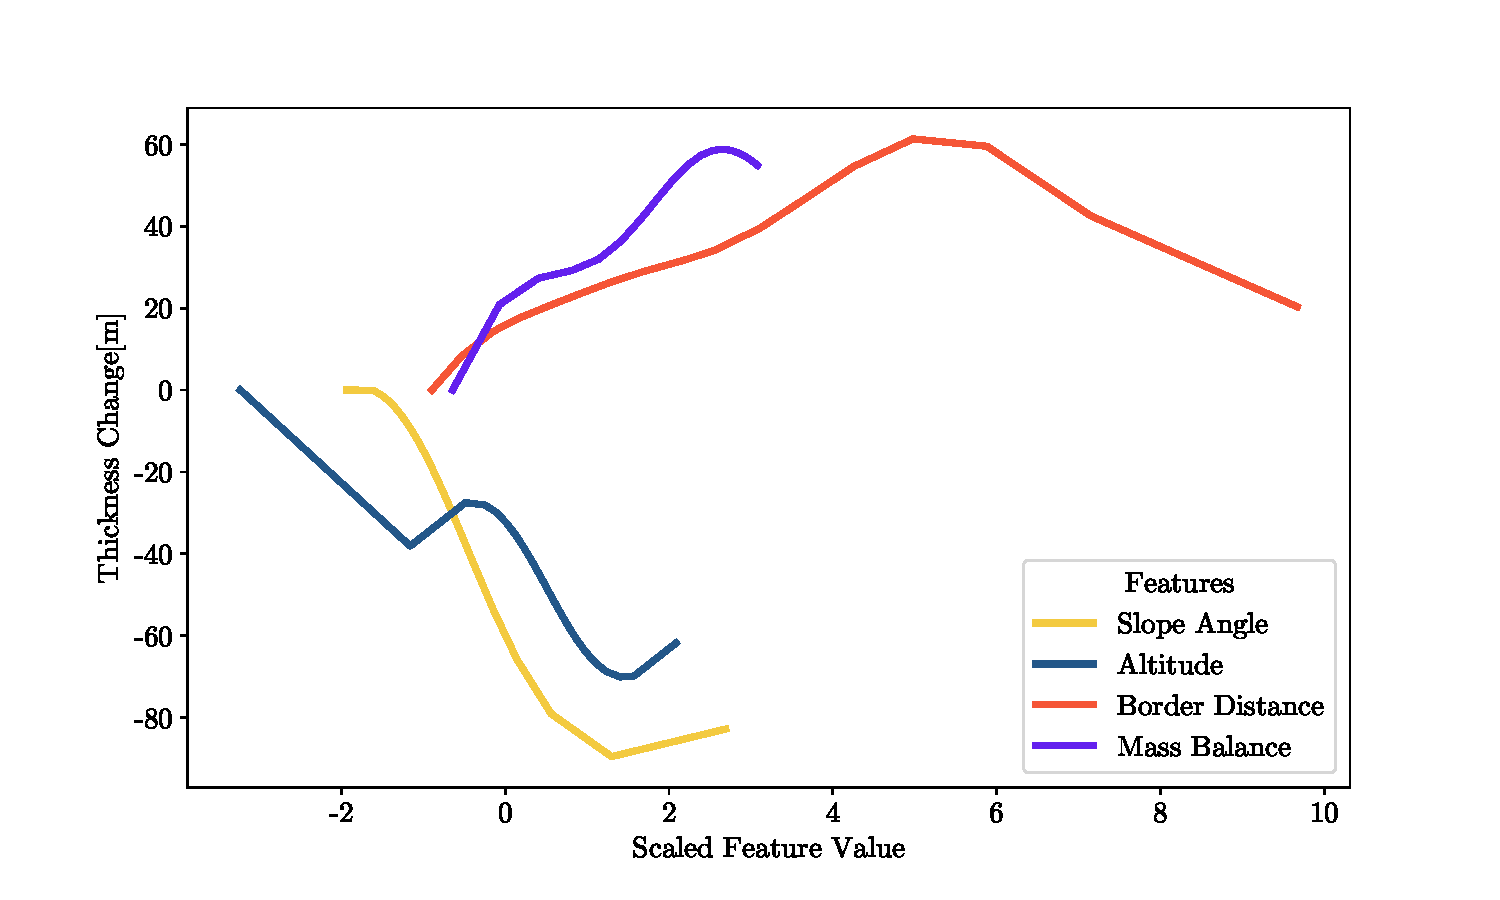
\includegraphics[width=1.\textwidth]{figures/SVR_low_thick_pdp.pdf}
	\caption{Partial plot analysis for glacier RGI60-11.01450 as predicted by the support vector regression model. The chart shows the change in ice thickness dependent on the change in values in the features used for training.}
	\label{fig:svr-pdp-low-thick}
\end{figure}

The support vector regression model presents a different problem when predicting the ice thickness distribution for some glaciers as RGI60-11.01450 which is a glacier with no thickness observations hence not used for training the models. The model seems unable to predict a reasonable ice thickness value and its distribution for this glacier. In particular the thickness value predicted for the glacier seems to be too small for such a large glacier and it is constant almost all over the whole glacier. The reason for this is probably the fact that for this particular glacier the linear mass balance greatly exceeds any value found in the training data-set as one could argue looking at Fig. \ref{fig:svr-pdp-low-thick}. This shows the partial dependence plot for the predictions of the support vector regression model for the input data for glacier RGI60-11.01450. Comparing it to Fig. \ref{fig:svr-pdp}, found in the results, showing the partial dependence plots for data inside the training data-set, and looking at the maximum values reached by  the linear mass balance for both cases it's clear that for RGI60-11.01450 this feature reaches values much large values. The model then has no way of knowing how to behave for such values as they are completely out of what it "learned" from the training process. Furthermore \ref{fig:svr-pdp} shows that the model learned that after a certain threshold for the linear mass balance the ice thickness decreases and the same behavior is visible for glacier RGI60-11.01450 as well, which led to ice thicknesses much lower than expected. After this decrease the model predicts no further ice thickness changes, as it had been trained with no information about linear mass balances as high as those computed for RGI60-11.01450, which leads to a constant low ice thickness distribution across the whole glacier.

Overall the performance of the predictions from the models doesn't seem to replicate the available observations in a particularly accurate manner. One of the causes for this, together with everything else mentioned above could be the temporal gap between when the observations were taken, which as seen in section \ref{survey-year}, has a rather high variance, and when the digital elevation model used to compute the features was compiled; glacier flows transform the glacier surface rather fast and thickness observations taken in one year could look rather different a couple of years later. Digital elevation models and observations measurements represent a single snapshot in a specific time and if the temporal gap between the two snapshots was lengthy the relationship between the geometrical features derived from the digital elevation model and the ice thickness could be compromised leading to poor training and predictions.

Also the accuracy of the observations in the GlaThiDa has not been taken into account at all and all the observations have been taken as the real value for the ice thickness.

\subsection{Feature importance}\label{disc-features}
For all models the most significant features when making predictions are the slope angle and the mass balance which was expected. However for the linear regression the most influential feature is the slope while for the support  vector machine is the mass balance. For the random forest regression the mass balance also seems like the most relevant feature when looking at the partial dependence plots (see Fig. \ref{fig:rfr-pdp}) and the permutation importance while the default feature importance accessible when training the model suggests the slope to be more influential in making the prediction.

When confronting the permutation importance heat-maps of the 3 models all of them present a drop in the coefficients for the sub-samples 5,14 and 19. This could be explained by the fact that the training data used in those sample are lacking information needed for the model to learn and therefore the importance of each feature used being lower. However recalling Eq. \ref{eq:perm} the permutation importance coefficient is the reduction in the score of model when preforming the permutation on the feature. As the score for the sub-samples already was low this reduction in score was probably less pronounced for those sub-samples. 

Finally looking at the partial dependence plots for the three models, non linear behavior of random forest and support vector regression, are clear. This can be an advantage of course when dealing with non linear dependencies. However while the linear model is able to predict any value even if completely out of the range of values used for training, the other two seem to struggle with those values. This doesn't mean that the linear model would necessarily lead to better prediction for those values but it shows how important is the training data-set for the other models. The best possible solution would be to train those models with data covering all the possible ranges of inputs and outputs.

\section{Alps volume comparison}\label{disc-alps}
A final interesting question is how the models used in this thesis compare with the model proposed by \citet{Farinotti2019} (ITMIX) which uses an ensemble of 5 physically based glacier models to model the glacier ice thickness of all glaciers in the world. The interesting comparison is that while those models are based on physical assumptions and  equation to predict the ice thickness, no assumption has been made in order for the machine learning models to make their predictions aside for choosing which input data to use to train them.
 
The data from \citet{Farinotti2019} comes as a list of all the glaciers with associated glacier volume as predicted by the ensemble of models. It is then possible to get an estimate of glacier ice volume for the whole world.
In order to keep thing simpler when training the machine learning models, the comparison has only been held for glaciers in the alpine regions and with the deletion of 36 glaciers for which it wasn't possible to compute the glaciers attributes needed for training.

\begin{table}[!tp]
	\centering
	\caption{Alpine glaciers total ice volumes in $m^3$ as predicted by the models. Differences are referred to the model from \citet{Farinotti2019} with the experiment called ITMIX}
	\begin{tabular}{|l|c|c|c|c|} 
		\cline{2-5}
		\multicolumn{1}{l|}{}                                                  & ITIMIX              & Linear Regression      & Random Forest           & Support Vector  \\ 
		\hline
		Volume [$m^3$]                                                                & 1.28$\times10^{11}$ & 1.40$\times10^{11}$    & 9.61$\times10^{10}$      & 9.58$\times10^{10}$        \\ 
		\hline
		\begin{tabular}[c]{@{}l@{}}Volume Difference\\from ITMIX [$m^3$]\end{tabular} & -                   & 1.25$\times10^{10}$    & -3.21$\times10^{10}$    & -2.82$\times10^{10}$      \\ 
		\hline
		Volume Difference \%                                                   &                 -    & 9.81\% & -22.1\% & -25.1\%   \\
		\hline
	\end{tabular}
	\label{tb:disc-vol}
\end{table}

The comparison table \ref{tb:disc-vol} shows the total volumes of ice for glaciers in the alpine region computed with the different machine learning models compared to the model from ITMIX. The linear regression model predicts the highest volume while the support vector regression predicts the lowest. Both random forest and support vector regression predict a total volume lower than the one predicted from ITMIX by over 22\%. These two models potentialy underestimate the total volume of alpine glaciers by over $\frac{1}{5}$ of the total ice volume. This difference is so big that it would make a very high impact in predicting, for example, see level rise especially if those differences were carried through for other glacier regions.

The reason for this discrepancies can be probably be imputed to the large spread in glacier sizes and attributes. The first important thing to notice is that according to the findings of \citet{Farinotti2019} 477 of the examined glacier in the alps are major outliers in the data-set when looking at their volume. In particular this means that these 477 glaciers have volumes larger than three times the inter-quartile volume range of all the alpine glaciers examined. This means that the vast majority of the glaciers in the alps are predicted to have much lower volumes compared to the largest glaciers. This makes correctly predicting the volume for these large glaciers extremely important when computing the total ice volume for the alpine glaciers. 477 glaciers represent the 12\% of all the alpine glaciers. According to ITMIX these 477 glacier account for 91.5\% of the total ice volume! Of these 477 glaciers 71 have at least one thickness observation in GlaThiDa which is 67\% of all the glaciers used for training the machine learning models. In theory then the training data-set is potentially well suited to learn about the glaciers with large volumes.  

\begin{figure}[!tp]
	\centering		  
	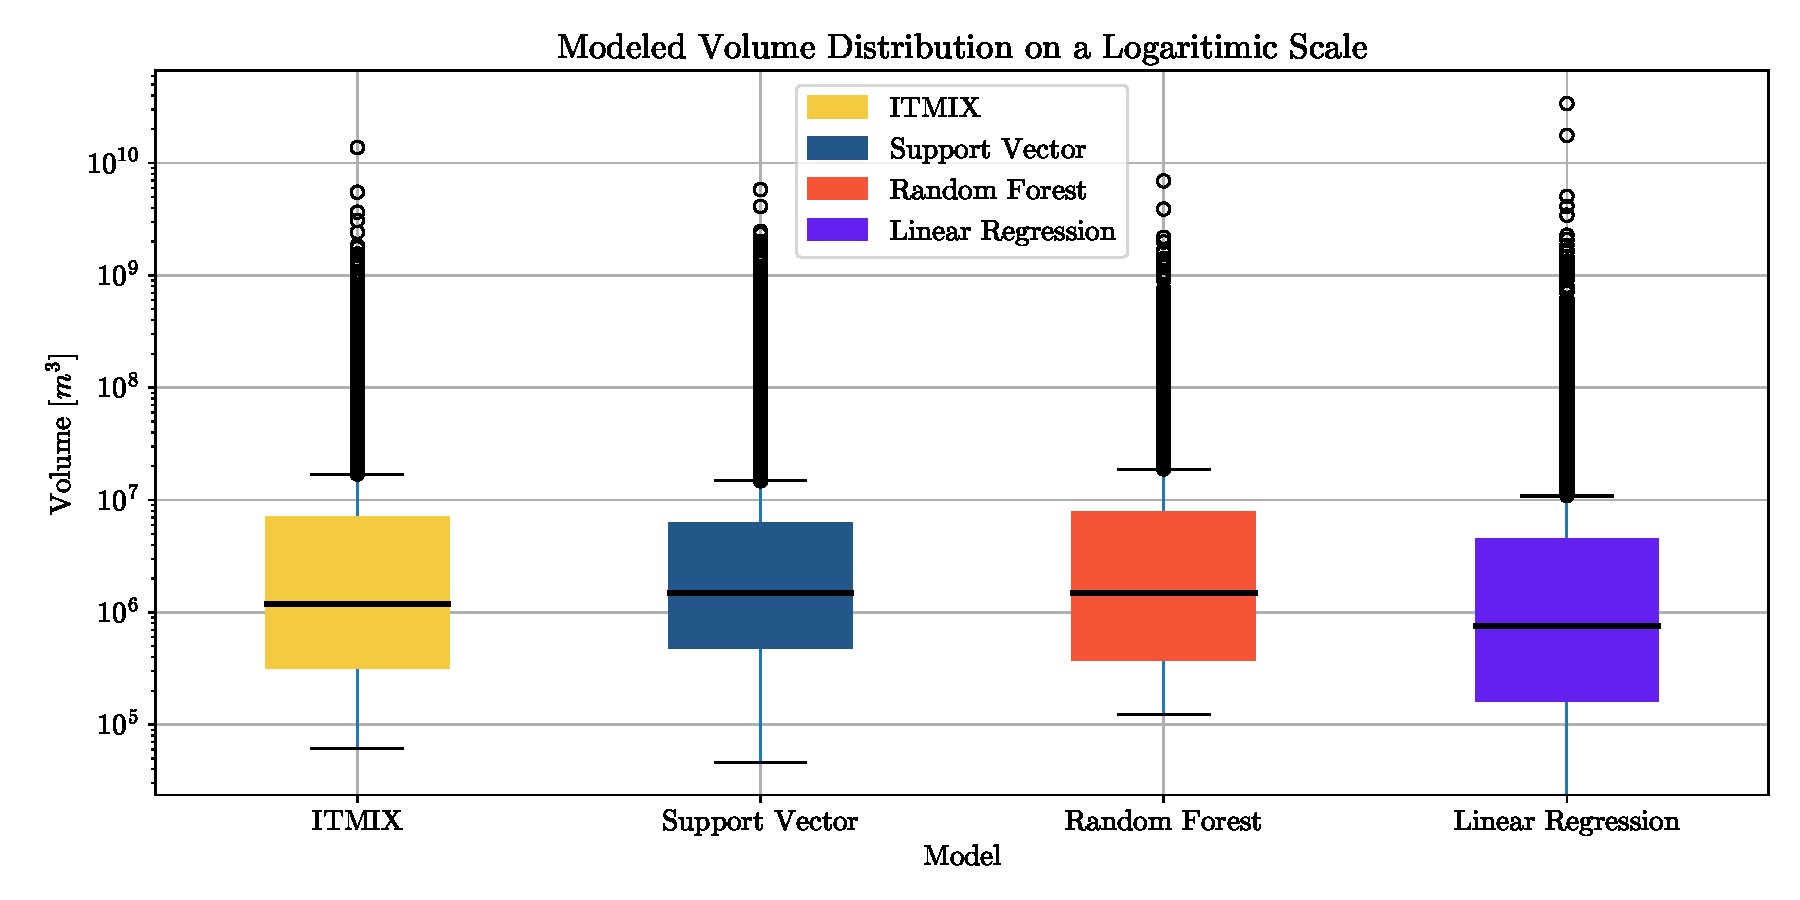
\includegraphics[width=1.\textwidth]{figures/vol_box.pdf}
	\caption{Distribution of alpine volumes as predicted by each model; note that the \textbf{y-axis is shown on a logarithmic scale}}
	\label{fig:vol-dist}
\end{figure}

Fig. \ref{fig:vol-dist} shows the volume distribution as predicted by all the models where the y-axis has been drawn on a logarithmic because of the large difference in volumes between smaller and larger glaciers. It is clear from the figure that both random forest and support vector regression predict an under-disperse volume distribution for large glaciers whereas the linear model predicts far larger volumes than the ITMIX for some glaciers. The support vector regression seems to have make more disperse predictions for smaller size glaciers while the random forest regression seem to have the lowest spread of all models.
random forest and support vector regression not being able to predict the ice thickness of large glaciers seems then to be the main cause for the differences in volume predictions between these two models and the one from \citet{Farinotti2019}.
The reason for this could be that larger glacier are underrepresented in the training data-set. However as just seen before this doesn't seem to be the case as 66\% of this data-set is composed by glaciers which are predicted to have large volumes.
Another reason could be that the number of observations with high ice thickness in the training data-set is low compared to the number of observations with lower ice thickness. The machine learning model would learn to predict better lower ice thickness than higher ones and it would be biased into predicting those. This is of course a normal behavior as machine learning models are not made to predict most of the data right and not the outliers. This is particularly evident for the random forest regression when looking at Fig. \ref{fig:rfr-map} where clearly the model is unable to predict ice thicknesses higher than 130$m$.
For the support vector regression though this is not necessarily the case as it seems like the model is able to predict ice thickness on the upper end of the ones found in the training data-set. However the model seems to be unable to predict a reasonable ice thickness and ice thickness distribution for some kind of glacier like RGI60-11.01450 as visible on the right of Fig. \ref{fig:svr-map}. As mentioned in section \ref{vol-dist}, this could be due to the fact that the input data used to make predictions fed to the algorithm while training don't fully represent the range of the ones found outside of them. This is clearly the case at least for the mass balance which also was the most influential feature in making predictions. Thirteen glaciers in the alps in fact are computed to have at least some mass balance values above the maximum one found in the training data-set. These thirteen glaciers alone account for almost 30\% of the total volume of the alpine glaciers and none of the models was trained to deal with this data. The total difference between the volume computed in the ITMIX and the one computed by the support vector regression for these thirteen glaciers, makes up almost 35\% of the total difference between the two models. 
Clearly not having the whole spectrum of possible input and output values available for training undermines the capability of making predictions of the machine learning algorithm. In this particular case this problem is enhanced by the fact that those values are the most important to the final result as of course bigger glaciers with higher ice thicknesses are the ones which most affect the total volume. 


%The discussion is the interpretation and evaluation of the results. It is a
%comparison of your results with previous findings. It provides the answer to the
%scientific questions raised in the introduction. It is the ``nerve center'' of a
%thesis, whereas the chapter Results may be seen as the ``heart''.
%
%Clearly separate between your own contributions and those of others. Provide
%rigorous citations of appropriate sources! Explicitly refer to specific results
%presented earlier. A certain amount of repetition is necessary. For
%example, the results presented in \ref{3sec:2} suggest that \dots. Order
%discussion items not chronologically but rather logically.
%
%The chapter Results answers the question: \emph{What} has been
%found? (Facts). The chapter Discussion answers the question: \emph{How} has the
%result to be interpreted? (Opinion).
%
%The most important message should appear in the first paragraph. The answer to
%the key question may appear in the first sentence: e.g., did your original idea
%work, or didn't it? The following questions may be answered in the discussion
%section:
%\begin{itemize}
%\item Why is the presented method simpler, better, more reliable than previous
%ones?
%\item What are its strengths and its limitations?
%\item How significant are the results?
%\item How trustworthy are the observations?
%\item Under which precondition/assumption and for which region are the
%results/method valid?
%\item Can the results be easily transferred to other regions or fields?
%\end{itemize}
